\section{Estimating Environmental-dependent Speciation \& Extinction Rates}

\subsection{Outline}

This tutorial describes how to specify a branching-process model with diversification rate correlated with an environmental variable in \RevBayes.
Diversification rates are assumed to be equal among all lineages but vary through time correlated with an environmental predictor variable.
Thus, this model can be used to test for correlations between diversification rates and environmental variables, such as \COO and temperature.
However, these tests are only to establish a correlation, not a causality.

As usual, we provide the probabilistic graphical model at the beginning of this tutorial.
Hopefully this will help you to get a better idea of all the variables in the model and their dependencies.
Our goal in this tutorial is to estimate the correlation coefficient between speciation and extinction rates to historical \COO measurements using Markov chain Monte Carlo (MCMC).


\subsection{Requirements}
We assume that you have read and hopefully completed the following tutorials:
\begin{itemize}
\item \href{https://github.com/revbayes/revbayes_tutorial/raw/master/tutorial_TeX/RB_Getting_Started/RB_Getting_Started.pdf}{Getting started}
\item \href{https://github.com/revbayes/revbayes_tutorial/raw/master/tutorial_TeX/RB_Basics_Tutorial/RB_Basics_Tutorial.pdf}{\Rev basics}
\item \href{https://github.com/revbayes/revbayes_tutorial/raw/master/tutorial_TeX/RB_DiversificationRate_Tutorial/RB_DiversificationRate_Tutorial.pdf}{Basic Diversification Rate Estimation}
\item \href{https://github.com/revbayes/revbayes_tutorial/raw/master/tutorial_TeX/RB_DiversificationRate_Episodic_Tutorial/RB_DiversificationRate_Episodic_Tutorial.pdf}{Diversification Rates Through Time}
\end{itemize}
Note that the \href{https://github.com/revbayes/revbayes_tutorial/raw/master/tutorial_TeX/RB_Basics_Tutorial/RB_Basics_Tutorial.pdf}{\Rev basics tutorial} introduces the basic syntax of \Rev but does not cover any phylogenetic models.
You may skip the \href{https://github.com/revbayes/revbayes_tutorial/raw/master/tutorial_TeX/RB_Basics_Tutorial/RB_Basics_Tutorial.pdf}{\Rev basics tutorial} if you have some familiarity with \R.
We tried to keep this tutorial very basic and introduce all the language concepts and theory on the way.
You may only need the \href{https://github.com/revbayes/revbayes_tutorial/raw/master/tutorial_TeX/RB_Basics_Tutorial/RB_Basics_Tutorial.pdf}{\Rev basics tutorial} for a more in-depth discussion of concepts in \Rev.

For this tutorial it is particularly important that you have read the two tutorials on diversification rate estimation: \href{https://github.com/revbayes/revbayes_tutorial/raw/master/tutorial_TeX/RB_DiversificationRate_Tutorial/RB_DiversificationRate_Tutorial.pdf}{Basic Diversification Rate Estimation tutorial} and \href{https://github.com/revbayes/revbayes_tutorial/raw/master/tutorial_TeX/RB_DiversificationRate_Episodic_Tutorial/RB_DiversificationRate_Episodic_Tutorial.pdf}{Diversification Rates Through Time tutorial}.
Specifically the \href{https://github.com/revbayes/revbayes_tutorial/raw/master/tutorial_TeX/RB_DiversificationRate_Episodic_Tutorial/RB_DiversificationRate_Episodic_Tutorial.pdf}{Diversification Rates Through Time tutorial} present the underlying diversification model and thus foundation for this tutorial.
Here we will build on the episodic diversification rate tutorial by modifying the prior model on diversification rates through time to depend on some environmental variable.

%%%%%%%%
%%   Data   %%
%%%%%%%%
\section{Data and files}

We provide the data file(s) which we will use in this tutorial.
You may want to use your own data instead.
In the \cl{data} folder, you will find the following files
\begin{itemize}
\item \cl{primates\_springer.tre}: Dated primates phylogeny including 369 out of 377 species from \cite{Springer2012}.
\end{itemize}


\impmark{Open the tree \cl{data/primates\_springer.tre} in \FigTree.}


\bigskip
\section{Environmental-dependent Diversification Rates}

The fundamental idea of this model is the question if diversification rates are correlated with an environmental variable.
Examples of environmental variables are \COO and temperature.
\begin{figure}[h!]
\centering
\fbox{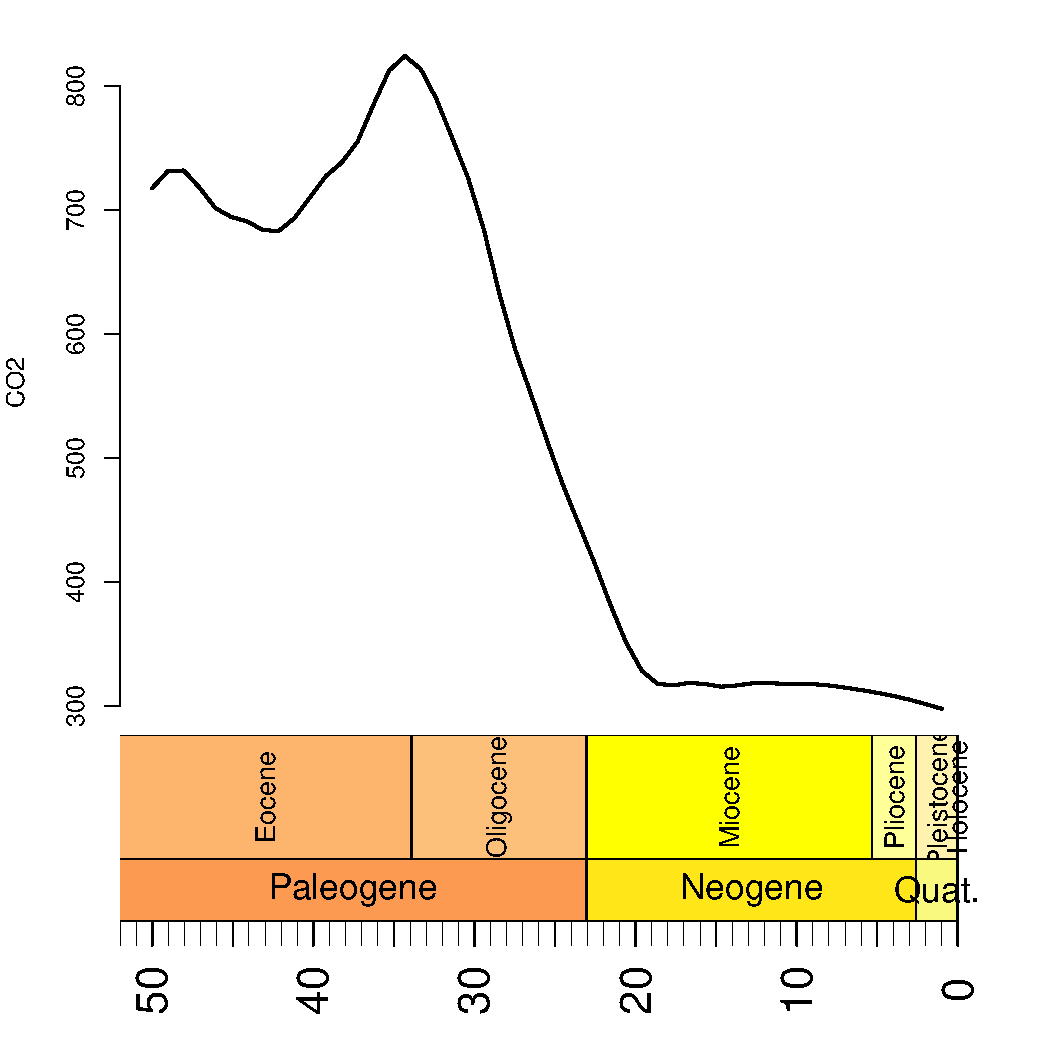
\includegraphics[width=0.6\textwidth]{\ResourcePath figures/Historical_CO2.pdf}}
\caption{\small Estimates of historical \COO values. These estimates are obtained from {\color{red}XXX}. The unit of \COO represents {\color{red}XXX}.}
\label{fig:CO2}
\end{figure}
Have a look at Figure~\ref{fig:CO2} which shows the historical value \COO in the last 50 million years.
We can clearly see that the \COO dropped drastically around 30 million years ago.

\begin{figure}[h!]
\centering
\fbox{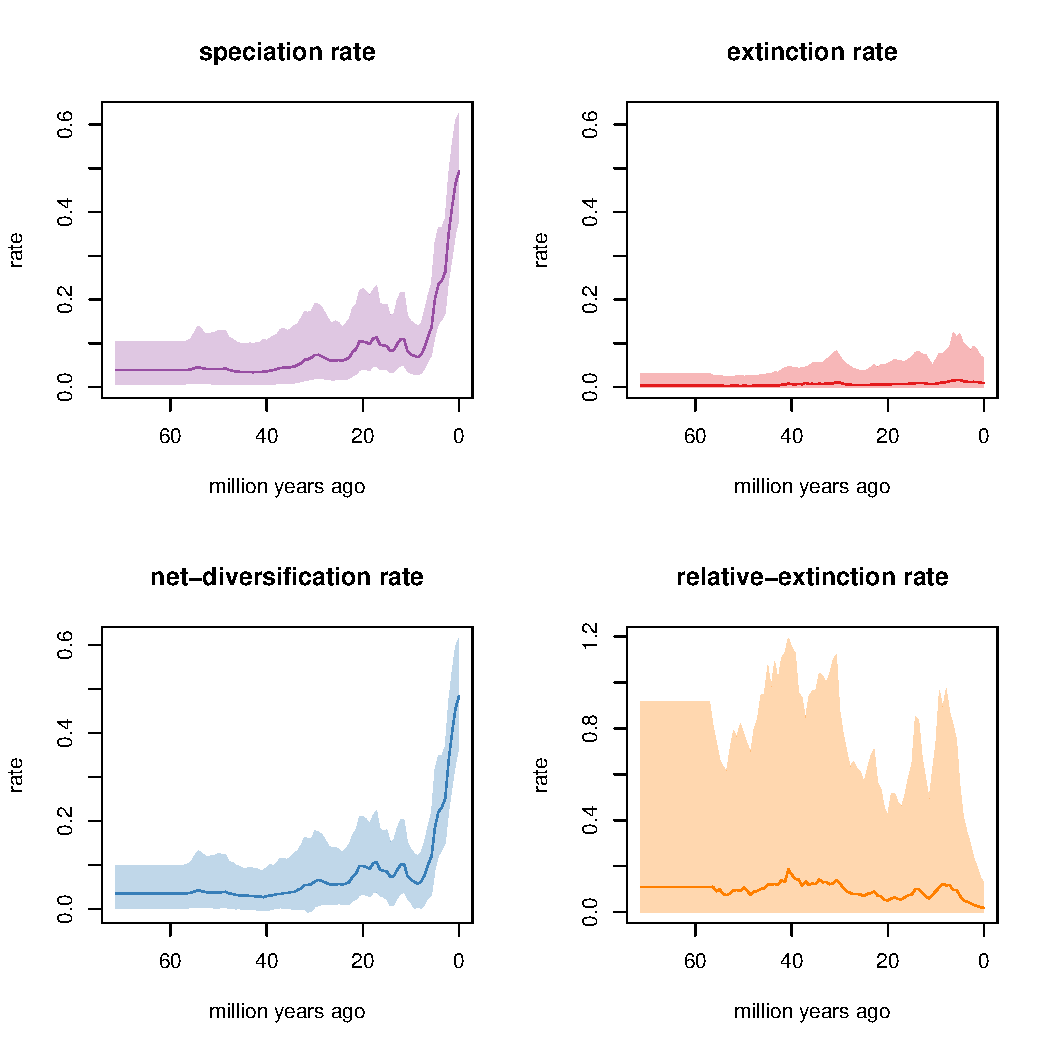
\includegraphics[width=0.6\textwidth]{\ResourcePath figures/EBD_Results.pdf}}
\caption{\small Estimated diversification rates through time. These estimates are taken from the episodic birth-death model with autocorrelated (Brownian motion) rate as described in the \href{https://github.com/revbayes/revbayes_tutorial/raw/master/tutorial_TeX/RB_DiversificationRate_Episodic_Tutorial/RB_DiversificationRate_Episodic_Tutorial.pdf}{Diversification Rates Through Time tutorial}.}
\label{fig:EBD_estimates}
\end{figure}
In our previous \href{https://github.com/revbayes/revbayes_tutorial/raw/master/tutorial_TeX/RB_DiversificationRate_Episodic_Tutorial/RB_DiversificationRate_Episodic_Tutorial.pdf}{Diversification Rates Through Time tutorial} we estimated diversification as shown in Figure~\ref{fig:EBD_estimates}.
We clearly see that diversification rates were not constant through time.
Now we wonder if perhaps the diversification rates are correlated with \COO.

We want to build on our episodic birth-death model so that our environmental correlation model collapses to the episodic birth-death model if there is no correlation.
Recall that we used a Brownian motion model on the log-transformed rates.
Hence, we assumed that the rates in the next time interval (epoch) have the current value as their expectation:
\begin{equation}
E[\log( \lambda(t) )] = \log( \lambda(t-\Delta t) )
\end{equation}
For the environmental dependent birth-death model, we have additional observation from the environmental variable.
Thus, we know how much the environmental variable changed between time intervals (epochs).
We can compute this change by taking the ratio between two consecutive measurements: $\frac{\text{CO}_2(t)}{\text{CO}_2(t-\Delta t)}$.
Hence, if the \COO double from one epoch to the next we would compute a change of 2.
This has the clear advantage that our computation is less sensitive to the unit and magnitude of the environmental variable.

Now let us assume that our diversification rates shift synchronously with the environmental variable if they are actually correlated.
Then we can express our expectation of the log-transformed diversification rate in the next time interval (epoch) as being equal the log-transform diversification rate in the current time interval plus the log-transformed change in the environmental variable:
\begin{equation}
E[\log( \lambda(t) )] = \log( \lambda(t-\Delta t) ) + \beta \times \log\left( \frac{\text{CO}_2(t)}{\text{CO}_2(t-\Delta t)} \right) \mbox{ .}
\end{equation}
Here we denote the correlation coefficient by $\beta$.
If $\beta > 0$ then there is a positive correlation between the speciation rate and \COO, that is, if the \COO increases then the speciation increases also.
If $\beta < 0$ then there is a negative correlation between the speciation rate and \COO, that is, if the \COO increases then the speciation decreases.
Finally, if $\beta = 0$ then there is no correlation and our model collapses to the episodic birth-death model.

In summary, we use a regression-like prior model for the speciation and extinction rate where the environmental variable (here \COO) is the predictor variable.
Specifically, we use a Brownian motion model for the log-transformed speciation and extinction rates where the expectation depends on the shift in the environmental variable.
Thus, our model can be considered as a Brownian motion model with drift where the drift parameter is the environmental variable.

We will now walk you through setting up this analysis in \RevBayes.

\subsection{Read the tree}

Begin by reading in the ``observed'' tree. 
{\tt \begin{snugshade*}
\begin{lstlisting}
T <- readTrees("data/primates_springer.tre")[1]
\end{lstlisting}
\end{snugshade*}}

From this tree, we get some helpful variables, such as the taxon information which we need to instantiate the birth-death process.
{\tt \begin{snugshade*}
\begin{lstlisting}
taxa <- T.taxa()
\end{lstlisting}
\end{snugshade*}}

Additionally, we initialize an iterator variable for our vector of moves and monitors.
{\tt \begin{snugshade*}
\begin{lstlisting}
mvi = 0
mni = 0
\end{lstlisting}
\end{snugshade*}}



\subsection{Set up the environmental data}

We take the \COO measurement from {\color{red}XXX} and store the values on a vector; one measurement (value) per interval.
{\tt \begin{snugshade*}
\begin{lstlisting}
var <- v(297.6, 301.36, 304.84, 307.86, 310.36, 312.53, 314.48, 316.31, 317.42, 317.63, 317.74, 318.51, 318.29, 316.5, 315.49, 317.64, 318.61, 316.6, 317.77, 328.27, 351.12, 381.87, 415.47, 446.86, 478.31, 513.77, 550.74, 586.68, 631.48, 684.13, 725.83, 757.81, 789.39, 813.79, 824.25, 812.6, 784.79, 755.25, 738.41, 727.53, 710.48, 693.55, 683.04, 683.99, 690.93, 694.44, 701.62, 718.05, 731.95, 731.56, 717.76)
\end{lstlisting}
\end{snugshade*}}
Then we specify the maximum age of the measurements.
This corresponds to the time of the last interval.
{\tt \begin{snugshade*}
\begin{lstlisting}
MAX_VAR_AGE = 50
\end{lstlisting}
\end{snugshade*}}
We will later use this maximum age to compute the times for each interval by assuming that each interval is equal in time.

Finally, we create a helper variable that specifies the number of intervals.
{\tt \begin{snugshade*}
\begin{lstlisting}
NUM_INTERVALS = var.size()-1
\end{lstlisting}
\end{snugshade*}}
This variable will help us to create the episodic diversification rate using a \cl{for}-loop.

\subsubsection{Setting up the time intervals}
In \RevBayes you actually have the possibility to specify unequal time intervals or even different intervals for the speciation and extinction rate.
This is achieved by providing a vector of times when each interval ends.
However, here we assume for simplicity that each interval has the same length because this is how we obtained our environmental data.
{\tt \begin{snugshade*}
\begin{lstlisting}
interval_times <- MAX_VAR_AGE * (1:NUM_INTERVALS) / NUM_INTERVALS
\end{lstlisting}
\end{snugshade*}}
This vector of times will be used for both the speciation and extinction rates.
Also, remember that the times of the intervals represent ages going backwards in time.


\subsection{Specifying the model}

\subsubsection{Priors on amount of rate variation}
We follow here exactly the prior specification as in the \href{https://github.com/revbayes/revbayes_tutorial/raw/master/tutorial_TeX/RB_DiversificationRate_Episodic_Tutorial/RB_DiversificationRate_Episodic_Tutorial.pdf}{Diversification Rates Through Time tutorial} because we want our model to collapse to the episodic birth-death if there is no correlation.

We start by specifying prior distributions on the rates.
Each interval-specific speciation and extinction rate will be drawn from a normal distribution.
Thus, we need a parameter for the standard deviation of those normal distributions.
We use an exponential hyperprior with rate 1.0 to estimate the standard deviation, but assume that all speciation rates and all extinction rates share the same standard deviation.
The motivation for an exponential hyperprior is that it has the highest probability density at 0 which would make the variance of rates between consecutive time intervals 0 and thus represent a constant rate process.
The data will tell us if there should be much variation in rates through time.
(You may want to experiment with this hyperprior if you are interested.)
{\tt \begin{snugshade*}
\begin{lstlisting}
speciation_sd ~ dnExponential(1.0)
extinction_sd ~ dnExponential(1.0)
\end{lstlisting}
\end{snugshade*}}
We apply a simple scaling move on each prior parameter.
{\tt \begin{snugshade*}
\begin{lstlisting}
moves[++mvi] = mvScale(speciation_sd,weight=5.0)
moves[++mvi] = mvScale(extinction_sd,weight=5.0)
\end{lstlisting}
\end{snugshade*}}


\subsubsection{Specifying the correlation coefficients}
Then we specify normal prior distributions on the correlation coefficient $\beta$ for the speciation and extinction rate.
Again, out total lack of prior knowledge, we will assume that the standard deviation of $\beta$ is $1.0$ and you may want to modify this value.
Nevertheless, this normal prior distribution is motivated by being centered at 0.0 (no correlation) and gives equal weight to positive and negative correlations.
{\tt \begin{snugshade*}
\begin{lstlisting}
beta_speciation ~ dnNormal(0,1.0)
beta_extinction ~ dnNormal(0,1.0)
\end{lstlisting}
\end{snugshade*}}
We apply simple sliding-window moves for the two correlation coefficients because they are defined on the whole real line.
{\tt \begin{snugshade*}
\begin{lstlisting}
moves[++mvi] = mvSlide(beta_speciation,delta=1.0,weight=10.0)
moves[++mvi] = mvSlide(beta_extinction,delta=1.0,weight=10.0)
\end{lstlisting}
\end{snugshade*}}
Additionally, we might be interested in the posterior probability that there is a positive correlation, $\mathbb{P}(\beta>0)$, or a negative correlation, $\mathbb{P}(\beta<0)$, respectively.
We achieve this using a deterministic variable that is 1 if $\beta<0$
{\tt \begin{snugshade*}
\begin{lstlisting}
speciation_corr_neg_prob := ifelse(beta_speciation < 0.0, 1, 0)
extinction_corr_neg_prob := ifelse(beta_extinction < 0.0, 1, 0)
speciation_corr_pos_prob := ifelse(beta_speciation > 0.0, 1, 0)
extinction_corr_pos_prob := ifelse(beta_extinction > 0.0, 1, 0)
\end{lstlisting}
\end{snugshade*}}
Note that in this model the probability of $\beta$ being 0.0 ($\mathbb{P}(\beta=0)=0$) because we are working with a prior and posterior \emph{density} on $\beta$ and thus any specific value, \EG 0.0, has a probability of 0.0.
We will circumvent this issue in the next chapter when we use reversible-jump MCMC to set $\beta$ specifically to 0.0.
Here you can also check that the posterior probability of \cl{speciation\_corr\_pos\_prob} equals 1-\cl{speciation\_corr\_neg\_prob}.

\subsubsection{Specifying correlated rates}
As we mentioned before, we will apply normal distributions as priors for each log-transformed rate.
We begin with the rate at the present which is our initial rate parameter.
The rates at the present will be specified slightly differently because they are not correlated to any previous rates.
This is because we are actually modeling rate-changes backwards in time and there is no previous rate for the rate at the present.

We use a uniform distribution between -10 and 10 because of our lack of prior knowledge on the diversification rate.
This actually means that we allow speciation and extinction rates between $e^{-10}$ and $e^10$ we should clearly cover the true values.
(Note that for diversification rate estimates $e^{-10}$ is virtually 0 since the rate is so slow).
{\tt \begin{snugshade*}
\begin{lstlisting}
log_speciation[1] ~ dnUniform(-10.0,10.0)
log_speciation[1] ~ dnUniform(-10.0,10.0)
\end{lstlisting}
\end{snugshade*}}
Notice that we store the diversification rate variables in vectors.
Storing the rate parameters in vectors will be useful and important later when we pass the rates into the birth-death process.

We apply simple sliding window moves for the rates.
Normally we would use scaling moves but in this case we work on the log-transformed parameters and thus sliding moves perform better.
(If you are keen you can test the differences.)
{\tt \begin{snugshade*}
\begin{lstlisting}
moves[++mvi] = mvSlide(log_speciation[1], weight=2)
moves[++mvi] = mvSlide(log_extinction[1], weight=2)
\end{lstlisting}
\end{snugshade*}}
Now we transform the diversification rate parameters into actual rates.
{\tt \begin{snugshade*}
\begin{lstlisting}
speciation[1] := exp( log_speciation[1] )
extinction[1] := exp( log_extinction[1] )
\end{lstlisting}
\end{snugshade*}}

Next, we specify the speciation and extinction rates for each time interval (\IE epoch).
This can be done efficiently using a \cl{for}-loop.
We will use a specific index variable so that we can easier refer to the rate at the previous interval.
Remember that we want to model the rates as a Brownian motion, which we achieve by specify a normal distribution as the prior distribution on the rates centered around the previous rate plus the change in the environmental variable (\IE the mean is equal to the previous rate plus the log-transformed ratio of the environmental variable divided by the previous value).
{\tt \begin{snugshade*}
\begin{lstlisting}
for (i in 1:NUM_INTERVALS) {
    index = i+1
    
    expected_speciation[index] := log_speciation[i] + beta_speciation * ln( var[index] / var[i] )
    expected_extinction[index] := log_extinction[i] + beta_extinction * ln( var[index] / var[i] )
    
    log_speciation[index] ~ dnNormal( mean=expected_speciation[index], sd=speciation_sd )
    log_extinction[index] ~ dnNormal( mean=expected_extinction[index], sd=extinction_sd )

    moves[++mvi] = mvSlide(log_speciation[index], weight=2)
    moves[++mvi] = mvSlide(log_extinction[index], weight=2)

    speciation[index] := exp( log_speciation[index] )
    extinction[index] := exp( log_extinction[index] )

}
\end{lstlisting}
\end{snugshade*}}
Finally, we apply moves that slide all values in the rate vectors, \IE all speciation or extinction rates. 
We will use an \cl{mvVectorSlide} move.
{\tt \begin{snugshade*}
\begin{lstlisting}
moves[++mvi] = mvVectorSlide(log_speciation, weight=10)
moves[++mvi] = mvVectorSlide(log_extinction, weight=10)
\end{lstlisting}
\end{snugshade*}}

Additionally, we apply a \cl{mvShrinkExpand} move which changes the spread of several variables around their mean.
{\tt \begin{snugshade*}
\begin{lstlisting}
moves[++mvi] = mvShrinkExpand( log_speciation, sd=speciation_sd, weight=10 )
moves[++mvi] = mvShrinkExpand( log_extinction, sd=extinction_sd, weight=10 )
\end{lstlisting}
\end{snugshade*}}
Both moves considerably improve the efficiency of our MCMC analysis.

\subsubsection{Incomplete Taxon Sampling}

We know that we have sampled 367 out of 377 living primate species. 
To account for this we can set the sampling parameter as a constant node with a value of 367/377.
For simplicity, and since almost all species have been sampled, we assume \emph{uniform} taxon sampling \citep{Hoehna2011,Hoehna2014a},
{\tt \begin{snugshade*}
\begin{lstlisting}
rho <- T.ntips()/377
\end{lstlisting}
\end{snugshade*}}


\subsubsection{Root age}

The birth-death process requires a parameter for the root age.
In this exercise we use a fix tree and thus we know the age of the tree.
Hence, we can get the value for the root from the \citet{Springer2012} tree.
{\tt \begin{snugshade*}
\begin{lstlisting}
root_time <- T.rootAge()
\end{lstlisting}
\end{snugshade*}}

\subsubsection{The time tree}

Now we have all of the parameters we need to specify the full episodic birth-death model. 
We initialize the stochastic node representing the time tree.
{\tt \begin{snugshade*}
\begin{lstlisting}
timetree ~ dnEpisodicBirthDeath(rootAge=T.rootAge(), lambdaRates=speciation, lambdaTimes=interval_times, muRates=extinction, muTimes=interval_times, rho=rho, samplingStrategy="uniform", condition="survival", taxa=taxa)
\end{lstlisting}
\end{snugshade*}}
You may notice that we explicitly specify that we want to condition on survival.
It is possible to change this condition to the \emph{time of the process} or \emph{the number of sampled taxa} too.

Then we attach data to the \cl{timetree} variable.
{\tt \begin{snugshade*}
\begin{lstlisting}
timetree.clamp(T)
\end{lstlisting}
\end{snugshade*}}

Finally, we create a workspace object of our whole model using the \cl{model()} function. 
{\tt \begin{snugshade*}
\begin{lstlisting}
mymodel = model(speciation)
\end{lstlisting}
\end{snugshade*}}

The \cl{model()} function traversed all of the connections and found all of the nodes we specified. 


\subsection{Running an MCMC analysis}

\subsubsection{Specifying Monitors}

For our MCMC analysis, we need to set up a vector of \textit{monitors} to record the states of our Markov chain. 
First, we will initialize the model monitor using the \cl{mnModel} function. This creates a new monitor variable that will output the states for all model parameters when passed into a MCMC function. 
{\tt \begin{snugshade*}
\begin{lstlisting}
monitors[++mni] = mnModel(filename="output/primates_EBD_Corr.log",printgen=10, separator = TAB)
\end{lstlisting}
\end{snugshade*}}

Additionally, we create four separate file monitors, one for each vector of speciation and extinction rates and for each speciation and extinction rate epoch (\IE the times when the interval ends).
We want to have the speciation and extinction rates stored separately so that we can plot them nicely afterwards.
{\tt \begin{snugshade*}
\begin{lstlisting}
monitors[++mni] = mnFile(filename="output/primates_EBD_Corr_speciation_rates.log",printgen=10, separator = TAB, speciation)
monitors[++mni] = mnFile(filename="output/primates_EBD_Corr_speciation_times.log",printgen=10, separator = TAB, interval_times)
monitors[++mni] = mnFile(filename="output/primates_EBD_Corr_extinction_rates.log",printgen=10, separator = TAB, extinction)
monitors[++mni] = mnFile(filename="output/primates_EBD_Corr_extinction_times.log",printgen=10, separator = TAB, interval_times)
\end{lstlisting}
\end{snugshade*}}

Finally, create a screen monitor that will report the states of specified variables to the screen with \cl{mnScreen}:
{\tt \begin{snugshade*}
\begin{lstlisting}
monitors[++mni] = mnScreen(printgen=1000, beta_speciation, beta_extinction)
\end{lstlisting}
\end{snugshade*}}

\subsubsection{Initializing and Running the MCMC Simulation}

With a fully specified model, a set of monitors, and a set of moves, we can now set up the MCMC algorithm that will sample parameter values in proportion to their posterior probability. The \cl{mcmc()} function will create our MCMC object:
{\tt \begin{snugshade*}
\begin{lstlisting}
mymcmc = mcmc(mymodel, monitors, moves)
\end{lstlisting}
\end{snugshade*}}

First, we will run a pre-burnin to tune the moves and to obtain starting values from the posterior distribution.
{\tt \begin{snugshade*}
\begin{lstlisting}
mymcmc.burnin(generations=10000,tuningInterval=200)
\end{lstlisting}
\end{snugshade*}}


Now, run the MCMC:
{\tt \begin{snugshade*}
\begin{lstlisting}
mymcmc.run(generations=50000)
\end{lstlisting}
\end{snugshade*}}

When the analysis is complete, you will have the monitored files in your output directory.
You can then visualize the rates through time using \R using our package \RevGadgets.
If you don't have the R-package \RevGadgets installed, or if you have trouble with the package, then please read the separate tutorial about the package.

Just start \R in the main directory for this analysis and then type the following commands:
{\tt \begin{snugshade*}
\begin{lstlisting}
library(RevGadgets)
tree <- read.tree("data/primates_Springer.tre")

# the CO2 values as a reference in our plot
co2 <- c(297.6, 301.36, 304.84, 307.86, 310.36, 312.53, 314.48, 316.31, 317.42, 317.63, 317.74, 318.51, 318.29, 316.5, 315.49, 317.64, 318.61, 316.6, 317.77, 328.27, 351.12, 381.87, 415.47, 446.86, 478.31, 513.77, 550.74, 586.68, 631.48, 684.13, 725.83, 757.81, 789.39, 813.79, 824.25, 812.6, 784.79, 755.25, 738.41, 727.53, 710.48, 693.55, 683.04, 683.99, 690.93, 694.44, 701.62, 718.05, 731.95, 731.56, 717.76)

MAX_VAR_AGE = 50
NUM_INTERVALS = length(co2)
co2_age <- MAX_VAR_AGE * (1:NUM_INTERVALS) / NUM_INTERVALS
predictor.ages <- co2_age
predictor.var <- co2

rev_out <- rev.process.div.rates(speciation_times_file = "output/primates_EBD_Corr_speciation_times.log",
                                 speciation_rates_file = "output/primates_EBD_Corr_speciation_rates.log",
                                 extinction_times_file = "output/primates_EBD_Corr_extinction_times.log",
                                 extinction_rates_file = "output/primates_EBD_Corr_extinction_rates.log",
                                 tree,
                                 burnin=0.25,numIntervals=100)
pdf("EBD_Corr.pdf")
par(mfrow=c(2,2))
rev.plot.div.rates(rev_out, predictor.ages=co2_age, predictor.var=co2, use.geoscale=TRUE)
dev.off()
\end{lstlisting}
\end{snugshade*}}

\impmark{The \Rev file for performing this analysis: \href{https://github.com/revbayes/revbayes_tutorial/raw/master/RB_DiversificationRate_Environmental_Tutorial/scripts/mcmc_EBD_Corr.Rev}{\cl{mcmc\_EBD.Rev}}.}


\subsection{A brief discussion on estimated diversification rates}
\begin{figure}
\subfloat[]{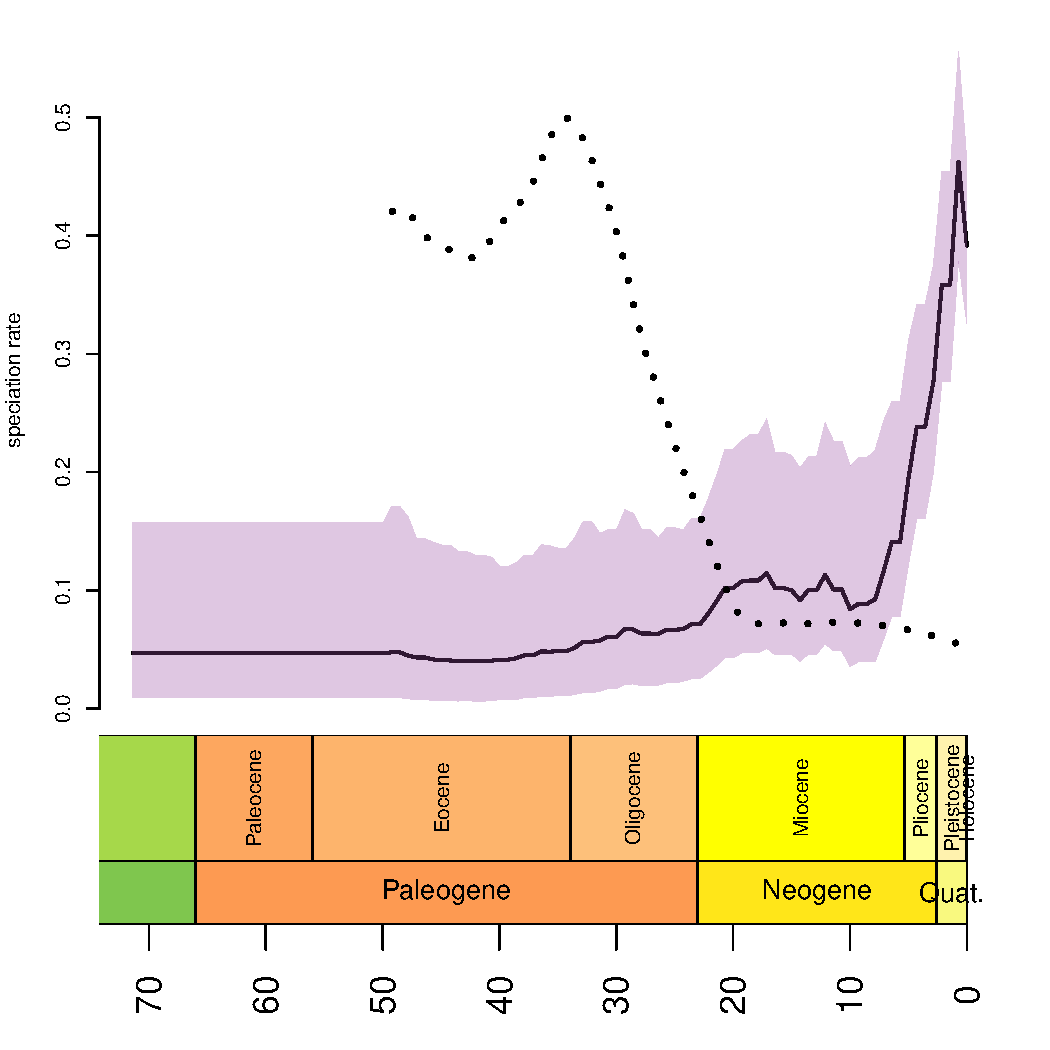
\includegraphics[width = 0.5\textwidth]{\ResourcePath figures/EBD_Corr_1.pdf}} 
\subfloat[]{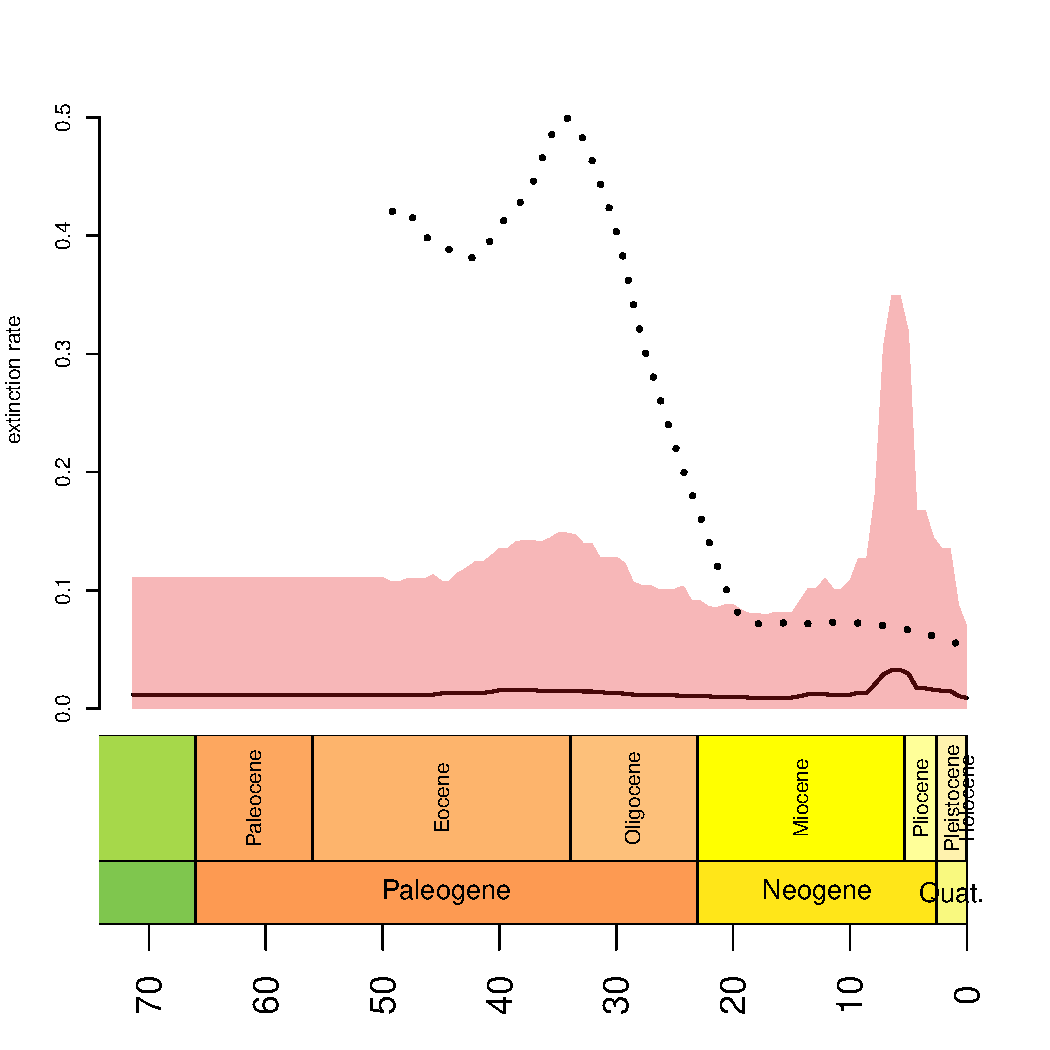
\includegraphics[width = 0.5\textwidth]{\ResourcePath figures/EBD_Corr_2.pdf}}\\
\subfloat[]{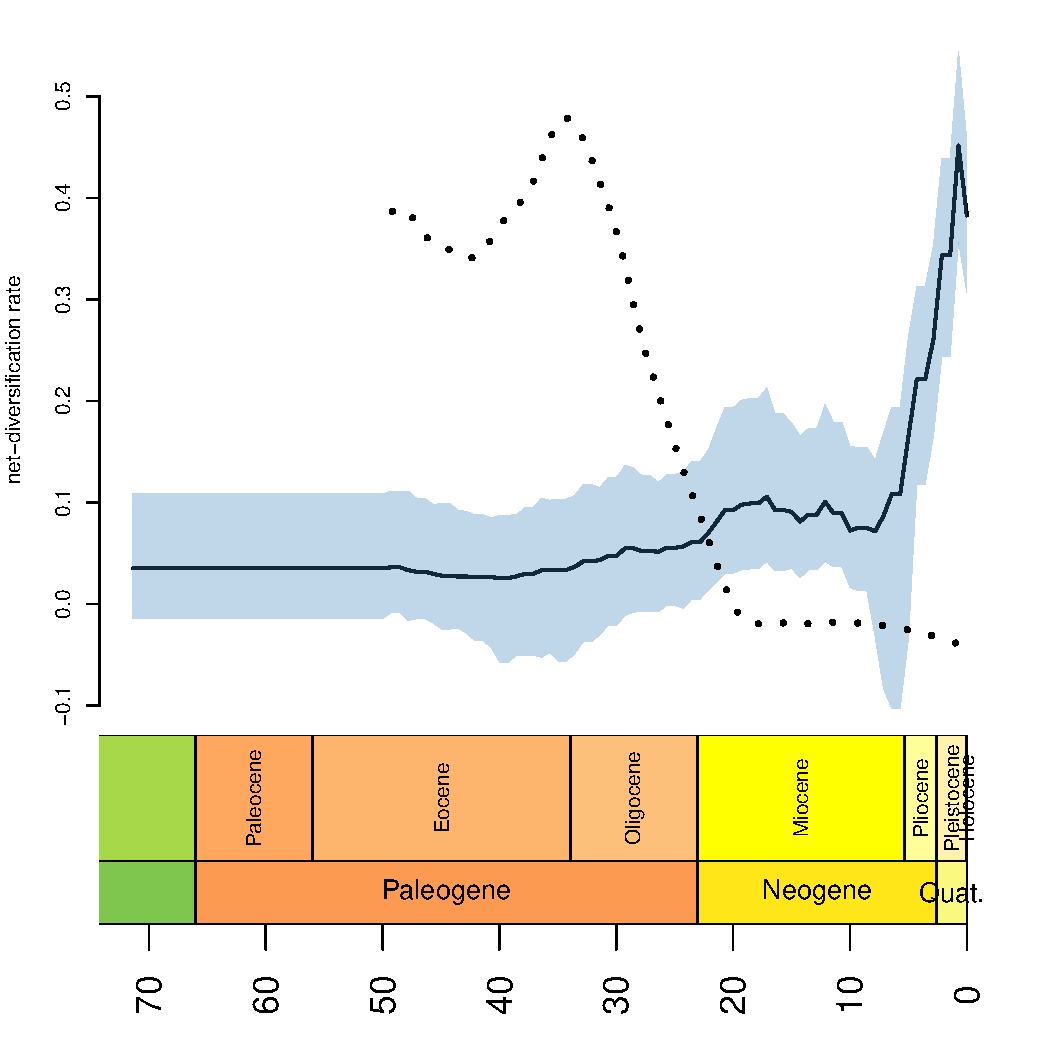
\includegraphics[width = 0.5\textwidth]{\ResourcePath figures/EBD_Corr_3.pdf}}
\subfloat[]{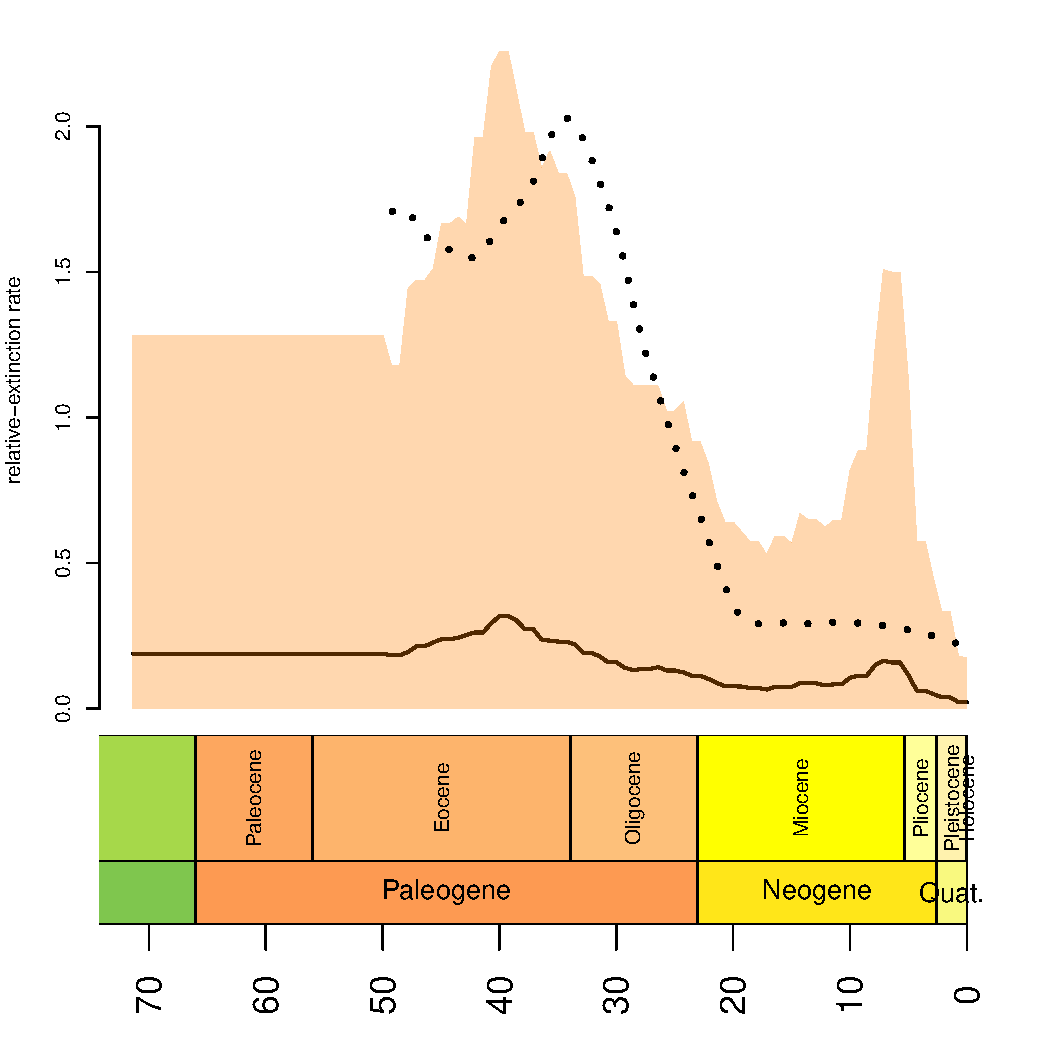
\includegraphics[width = 0.5\textwidth]{\ResourcePath figures/EBD_Corr_4.pdf}} 
\caption{\small Resulting diversification rate estimations}
\label{fig:EBD_Results}
\end{figure}

Figure~\ref{fig:EBD_Results} shows the estimated diversification rates through time and the \COO.
If you compare these estimates with Figure~\ref{fig:EBD_estimates} then you may notice that the diversification rate estimate are virtually identical.
This is a good sign for the analysis because it shows that the information in the estimates comes from the data (the tree in this case) and not from the assumed model.
Thus, we are not artificially forcing the diversification rates to follow our environmental variable but instead estimate if there is a correlation.
Small deviation between the estimated rates under the different analyses are expected because there will be some interaction between the environmental variable and the diversification rate estimates.
Additionally, the uncertainty in estimated diversification rates through time is large und minor changes are within this uncertainty. 


\subsection{Exercise 1}

\begin{itemize}
\item Run an MCMC simulation to estimate the posterior distribution of the speciation rate and extinction rate.
\item Visualize the rate through time using \R.
\item Open the file \cl{output/primates\_EBD\_Corr.log} in \Tracer. What is the estimated probability that $\beta<0$? You'll find the estimate in the variable \cl{speciation\_corr\_neg\_prob}.
\item We specified a normal prior with mean 0 on $\beta$ and thus used a prior probability of 0.5 that $\beta<0$. Now you can use the posterior ratio divided by the prior ratio to compute the Bayes factor. What is the Bayes factor support for or against a positive correlation between the speciation rate and \COO?
\item Similarly, is there support for a positive or negative correlation between the extinction rate and \COO?
\end{itemize}




\bigskip
\section{Testing for correlation using reversible-jump MCMC}

In the previous exercise we wanted that our model collapses to the episodic birth-death process if there is no environmental correlation.
We achieved this by setting up our prior model so that if $\beta=0$ the model collapses.
However, we also used a normal prior distribution with mean 0.0 and standard deviation 1.0 for $\beta$.
Thus, we implicitly specified that $\beta$ being exactly 0.0 has probability 0.0 because every specific value of a continuous distribution has a 0.0 probability despite having a positive probability density.
For example, you might notice that you will never sample in your MCMC run the value 0.0 exactly although we might sample values that are close to 0.0.

Now we want to use reversible jump MCMC to test specifically if the hypothesis $\beta=0$ is rejected.
Remember that reversible jump MCMC can estimate the posterior probability for different models.
The first model will be that $\beta=0$ and the second model will be that $\beta \sim \text{norm}(0,1)$.
Then we can simply compute Bayes factors by computing the posterior ratio divided by the prior ratio to assess the support for either model.

In \RevBayes we have a very flexible way to specify a reversible-jump MCMC.
We can provide any constant value and distribution to the distribution \cl{dnReversibleJumpMixture}.
This will mean that the value, \cl{beta\_speciation} and \cl{beta\_extinction}, will either take on the constant value or drawn from the base-distribution.
{\tt \begin{snugshade*}
\begin{lstlisting}
beta_speciation ~ dnReversibleJumpMixture(constantValue=0.0, baseDistribution=dnNormal(0,1.0), p=0.5)
beta_extinction ~ dnReversibleJumpMixture(constantValue=0.0, baseDistribution=dnNormal(0,1.0), p=0.5)
\end{lstlisting}
\end{snugshade*}}
Additionally we also need a specific move that switches if the value is equal to the constant value or drawn from the base-distribution.
This is where we use the reversible-jump move \cl{mvRJSwitch}.
{\tt \begin{snugshade*}
\begin{lstlisting}moves[++mvi] = mvRJSwitch(beta_speciation, weight=5)
moves[++mvi] = mvRJSwitch(beta_extinction, weight=5)
\end{lstlisting}
\end{snugshade*}}
Now we can also monitor for convenience what the probability of \cl{beta\_speciation} and \cl{beta\_extinction} being 0.0 is.
We will set this up by a deterministic variable that will be 1.0 if $\beta \neq 0$ and will be 0.0 if $\beta = 0.0$.
Thus the two variables \cl{speciation\_corr\_prob} and \cl{extinction\_corr\_prob} represent the probability that there is a correlation between the speciation rate or the extinction rate and \COO.
{\tt \begin{snugshade*}
\begin{lstlisting}
speciation_corr_prob := ifelse(beta_speciation == 0.0, 0, 1)
extinction_corr_prob := ifelse(beta_extinction == 0.0, 0, 1)
\end{lstlisting}
\end{snugshade*}}

These are the only necessary changes to the above analysis to run a reversible-jump MCMC.

\subsection{Exercise 2}

\begin{itemize}
\item Make a copy of the script \cl{mcmc\_EBD\_Corr.Rev} and call it \cl{mcmc\_EBD\_Corr\_RJ.Rev}.
\item Replace the prior distribution on \cl{beta\_speciation} and \cl{beta\_extinction} to use the \cl{dnReversibleJumpMixture} instead.
\item Also add the new moves \cl{mvRJSwitch} and deterministic variables  \cl{speciation\_corr\_prob} and \cl{extinction\_corr\_prob}.
\item Don't forget to change the output filenames in the monitors, \EG add \cl{\_RJ} to the name.
\item Run the reversible-jump MCMC analysis.
\item Open the file \cl{output/primates\_EBD\_Corr\_RJ.log} in \Tracer. What is the estimated probability that $\beta=0$? You'll find the estimate in the variable \cl{speciation\_corr\_prob}.
\item We specified a prior probability of 0.5 on $\beta$ being fixed to 0.0. Now you can use the posterior ratio divided by the prior ratio to compute the Bayes factor. What is the Bayes factor support for or against any correlation between the speciation rate and \COO?
\item Similarly, is there support for a positive or negative correlation between the extinction rate and \COO?
\end{itemize}

\bibliographystyle{sysbio}
\bibliography{\GlobalResourcePath refs}
